\chapter{分子植物生理学与胁迫响应}\label{ch:b3:plant-molecular-physiology}

在暗柜中生长的菜豆幼苗苍白而细弱：
一根长长的白色茎，顶端一个弯钩，
两片皱缩的黄色叶片。把它移到窗边，
不到一天，它便停止伸长，弯钩伸直，
叶片展开并转绿——同一套基因，
却成了另一个生物体。它等待的不是能量，
而是信息。一个被单一蛋白质吸收的红光光子，
告诉它已抵达光照之处；红光与远红光的比值，
告诉它邻近的叶片是否在头顶；夜的长短，
告诉它季节；根部水势的下降、一阵风、
叶片上细菌的鞭毛蛋白，每一种信号都由受体探测，
转化为化学信号，再以某些基因是否表达、
哪些细胞生长的改变作出应答。植物无法逃离环境，
它只能读取环境，并重塑自身。
本章讨论的正是这种“读取”：光受体，\omterm{def:b3:endocrinology:hormone}{激素}及其在分子尺度上的作用方式，
对干旱、盐、冷和热的响应，
以及植物在没有任何可移动细胞的情况下演化出的双层免疫系统。

\section{读取光信号}

\begin{definition}[光受体]\label{def:b3:plant-molecular-physiology:photoreceptors}
\index{光敏色素}\index{隐花色素}\index{向光素}\index{光形态建成}\index{黄化}
植物借助三类蛋白质感知光，三者均不含
叶绿素。\emph{光敏色素}是二聚体，含胆色素辅基，
红光（\qty{660}{nm}）使其由无活性的\emph{Pr}型转为
有活性的\emph{Pfr}型，远红光（\qty{730}{nm}）使其逆转；Pfr
进入细胞核，标记一类转录因子 PIF 以供降解，
从而释放光下发育的相关基因；
黑暗中 Pfr 缓慢逆转。\emph{隐花色素}（蓝光，
\qty{450}{nm}）是与 DNA 修复酶相关的黄素蛋白，
调控去黄化、生物钟与开花；\emph{向光素}
（蓝光）是膜上的激酶，引导向光弯曲、
\omterm{prop:b3:plant-molecular-physiology:stomata}{气孔}开放与叶绿体的移动。黑暗中的幼苗
处于\emph{黄化}状态——下胚轴细长，子叶闭合，无叶绿素，
全部资源都用于抵达地表；光照
使其转入\emph{光形态建成}，此转换由 Pfr 与隐花色素共同作用，
使单一阻遏复合体（COP1）失活而触发，
该复合体在黑暗中会降解光程序的
转录因子。由此，光被读取两次：作为能量，
由叶绿体读取；作为信号，由对小一百万倍的
光子通量敏感的受体读取。
\end{definition}

\begin{proposition}[光敏色素光平衡]\label{prop:b3:plant-molecular-physiology:photoequilibrium}
\index{光平衡}\index{红光与远红光比值}\index{避荫}
在持续光照下，Pr 与 Pfr 相互转化，直至
两个光转换速率达到平衡：设 $k_{1}$ 为 Pr $\to$ Pfr
的速率（与红光通量成正比），$k_{2}$ 为 Pfr $\to$ Pr
的速率（与远红光通量成正比，另加少量来自红光，因为
Pfr 也吸收红光），则活性形式的比例为
\[
\varphi = \frac{[\text{Pfr}]}{[\text{Pfr}] + [\text{Pr}]} = \frac{k_{1}}{k_{1} + k_{2}},
\]
它与总通量无关，仅由光的\emph{\omterm{prop:b3:plant-molecular-physiology:photoequilibrium}{红光与远红光比值}}
$\zeta$ 决定。纯红光时 $\varphi \approx 0.87$（Pfr
也吸收部分红光），纯远红光时为 $0.03$；自然日光下 $\zeta \approx
1.15$ 时约为 $0.55$，而叶层冠下的光，
叶绿素已吸收了红光、透过了远红光，其
$\zeta \approx 0.2$，$\varphi \approx 0.2$。植物以其
$\varphi$ 判断周围有无邻居：其值低时便触发
\emph{\omterm{prop:b3:plant-molecular-physiology:photoequilibrium}{避荫}}反应——茎伸长、叶片上举、
提早开花、分枝减少——其途径是 Pfr 不再降解的
PIF。农田密植的作物即为\omterm{prop:b3:plant-molecular-physiology:photoequilibrium}{避荫}型群体；
绿色革命中的矮秆小麦对此信号不敏感，
将节省下来的生长量全部转入籽粒。
\end{proposition}
\begin{proof}
$\mathrm{d}[\text{Pfr}]/\mathrm{d}t = k_{1}[\text{Pr}] - k_{2}[\text{Pfr}]$
在 $[\text{Pr}] + [\text{Pfr}] = P$ 固定的条件下，稳态时有
$k_{1}(P - [\text{Pfr}]) = k_{2}[\text{Pfr}]$，由此得 $\varphi = k_{1}/
(k_{1} + k_{2})$。两个速率都与入射通量成正比，因此
按比例改变光照会同时改变两者，$\varphi$ 不变；只有
光谱组成起作用。趋近稳态的速率为
$k_{1} + k_{2}$——日光下为秒级，黄昏时为分钟级；而 Pfr 的暗逆转
（半衰期为数小时）决定了
夜间残留的比例。
\end{proof}

\begin{omfigure}
\begin{tikzpicture}[every node/.style={font=\scriptsize}, >=stealth]
  \node[draw, very thick, omDef, fill=omDef!15, rounded corners, minimum width=1.6cm, minimum height=0.9cm] (pr) at (0,0) {Pr（无活性）};
  \node[draw, very thick, omThm, fill=omThm!15, rounded corners, minimum width=1.6cm, minimum height=0.9cm] (pfr) at (4.2,0) {Pfr（有活性）};
  \draw[->, very thick, red!70!black] (pr.north east) to[bend left=25] node[above] {红光，\qty{660}{nm}} (pfr.north west);
  \draw[->, very thick, red!40!black] (pfr.south west) to[bend left=25] node[below] {远红光，\qty{730}{nm}} (pr.south east);
  \draw[->, thick, gray] (pfr.south) ++(0.5,-0.15) to[bend left=40] node[right, font=\tiny, gray] {暗逆转，数小时} ++(-0.3,-0.9);
  \draw[->, thick] (pfr.east) -- ++(1.0,0) node[right, align=left] {进入细胞核：\\PIF 降解，COP1 关闭；\\光下生长程序开启};
  \begin{scope}[shift={(0,-4.6)}]
  \begin{axis}[
    width=0.55\linewidth, height=4.6cm,
    axis x line=bottom, axis y line=left,
    xmin=0, xmax=2.5, ymin=0, ymax=1,
    xlabel={红光与远红光比值 $\zeta$}, ylabel={$\varphi = $ Pfr 比例},
    xlabel style={font=\scriptsize, at={(axis description cs:0.5,-0.15)}, anchor=north}, ylabel style={font=\scriptsize},
    tick label style={font=\scriptsize}, xtick={0.2,0.5,1.15,2}, xticklabels={0.2,0.5,1.15,2}, ytick={0.2,0.55,0.87},
    clip=false,
  ]
  \addplot[very thick, omDef, domain=0:2.5, samples=80] {0.87*x/(x+0.6)};
  \draw[dashed, gray] (axis cs:0.2,0) -- (axis cs:0.2,0.22) -- (axis cs:0,0.22);
  \draw[dashed, gray] (axis cs:1.15,0) -- (axis cs:1.15,0.57) -- (axis cs:0,0.57);
  \node[font=\tiny, anchor=west, align=left] at (axis cs:0.25,0.12) {冠层之下：\\避荫};
  \node[font=\tiny, anchor=south west] at (axis cs:1.2,0.62) {开阔日光};
  \node[font=\tiny, anchor=north west, omDef, align=left] at (axis cs:1.6,0.45) {经验拟合，\\$\varphi \approx 0.87\,\zeta/(\zeta + 0.6)$};
  \end{axis}
  \end{scope}
\end{tikzpicture}

{\small \omterm{def:b3:plant-molecular-physiology:photoreceptors}{光敏色素}开关。红光使其成为活性形式，
远红光使其失活，黑暗中则缓慢逆转；活性形式的稳态比例
取决于光的颜色平衡，而非其亮度，
这正是幼苗得以知道上方有叶片遮挡的原因。}
\end{omfigure}

\begin{proof}[证据]
博斯威克、亨德里克斯及其同事（1952 年）用短暂闪光照射生菜种子：
红光使种子萌发，随后照射远红光则抵消这一效应，
再照红光又使其恢复萌发，如此交替十余次——
最后一次闪光起决定作用，这是可逆色素的特征。他们随后
（1959 年）提取出一种蓝色蛋白质，它在红光和远红光照射下吸收光谱
发生变化。后来研究表明，黑暗中生长的幼苗整套发育程序
依赖于一个阻遏蛋白：缺失 COP1 的突变体在完全黑暗中发育，仿佛处于光照之下，
植株矮小，且已具备转绿的条件；
而缺失\omterm{def:b3:plant-molecular-physiology:photoreceptors}{光敏色素}和\omterm{def:b3:plant-molecular-physiology:photoreceptors}{隐花色素}的突变体
在光照下仍保持\omterm{def:b3:plant-molecular-physiology:photoreceptors}{黄化}状态。
\end{proof}

\begin{omfigure}
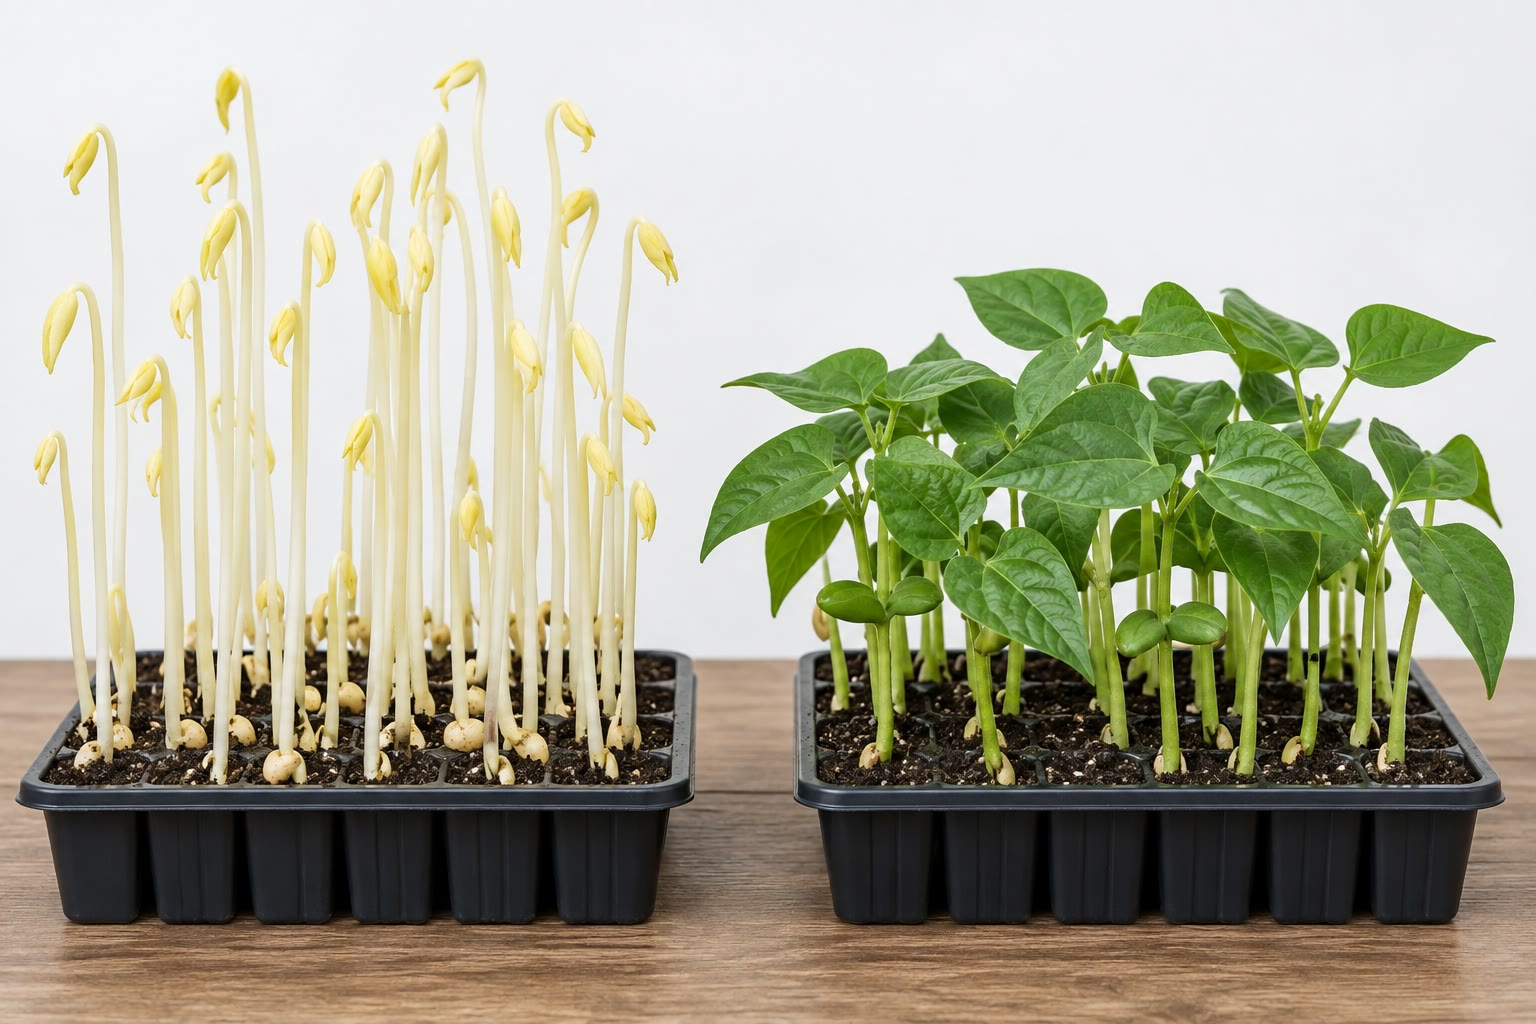
\includegraphics[width=0.56\linewidth]{images/book5/ai/b5-22-etiolated-seedlings.jpg}

{\small 黑暗与光照中生长的幼苗：基因组相同，
发育程序却不同，其差别源于一个红光光子
被\omterm{def:b3:plant-molecular-physiology:photoreceptors}{光敏色素}吸收。}
\end{omfigure}

\section{分子尺度上的激素}

\begin{definition}[植物激素及其受体]\label{def:b3:plant-molecular-physiology:hormones}
\index{生长素}\index{TIR1}\index{赤霉素}\index{DELLA}\index{脱落酸}\index{乙烯}\index{细胞分裂素}\index{油菜素甾醇}
本科一年级分册介绍了植物\omterm{def:b3:endocrinology:hormone}{激素}的作用，这里讲的是它们如何
被“接收”。多种\omterm{def:b3:endocrinology:hormone}{激素}通过\emph{受调控的降解}发挥作用。
\emph{生长素}（吲哚-3-乙酸）与 F-box 蛋白
\emph{TIR1}结合，使其与 Aux/IAA 阻遏蛋白结合在一起，
随后阻遏蛋白被泛素化并经蛋白酶体降解：原先被其抑制的生长素响应基因
在数分钟内即被开启——\omterm{def:b3:endocrinology:hormone}{激素}是一种分子“胶水”，
而受体本身即是降解机器的一部分。
\emph{赤霉素}以相同方式作用于控制生长的 \emph{DELLA} 阻遏蛋白，
通过其受体 GID1 发挥作用：绿色革命中的矮秆小麦和水稻
携带的 DELLA 蛋白无法被降解，因而
无论合成多少赤霉素，植株都保持矮小。\emph{\omterm{def:b3:plant-molecular-physiology:immunity}{茉莉酸}}
遵循相同逻辑，作用于 JAZ 阻遏蛋白。\emph{脱落酸}
（ABA），干旱和休眠的\omterm{def:b3:endocrinology:hormone}{激素}，与 PYR/PYL 受体结合，
受体随后抑制磷酸酶（PP2C），释放出一种激酶
（SnRK2），后者使离子通道和转录因子磷酸化——
这是一种双重负调控，使反应变得陡峭。\emph{乙烯}是一种
气体，它与内质网膜上含铜的受体结合；在缺乏乙烯时，
这些受体会主动抑制相应反应，结合乙烯则使其失活，于是
成熟、\omterm{def:b3:cell-cycle-apoptosis:other}{衰老}和胁迫相关基因随之开启。\emph{细胞分裂素}
通过组氨酸激酶类受体发挥作用，类似于细菌的\omterm{def:b3:bacteriology:quorum}{双组分系统}；
\emph{油菜素甾醇}是植物的甾体\omterm{def:b3:endocrinology:hormone}{激素}，通过
一种细胞表面受体激酶而非\omterm{def:b3:endocrinology:hormone}{核受体}发挥作用——它是唯一
在细胞表面被“接收”的甾体\omterm{def:b3:endocrinology:hormone}{激素}。植物没有腺体：每种\omterm{def:b3:endocrinology:hormone}{激素}
在需要之处合成，或由特定载体运送，
其浓度由合成、结合
和降解在局部调控。
\end{definition}

\begin{theorem}[生长素的化学渗透极性运输]\label{thm:b3:plant-molecular-physiology:auxin}
\index{极性生长素运输}\index{PIN 蛋白}\index{阴离子捕获}
吲哚-3-乙酸是一种弱酸，$\mathrm{p}K_{a} = 4.75$。在
pH~$5.5$ 的细胞壁空间中，相当大的比例为中性的
IAAH，可以穿过膜扩散；在 pH~$7.2$ 的细胞质溶胶中，
几乎全部为阴离子 IAA$^{-}$，无法通过扩散离开。在中性形式跨膜
达到平衡时，细胞内外总\omterm{def:b3:plant-molecular-physiology:hormones}{生长素}之比
为
\[
\frac{[\text{IAA}]_{\text{内}}}{[\text{IAA}]_{\text{外}}}
= \frac{1 + 10^{\,\mathrm{pH}_{\text{内}} - \mathrm{p}K_{a}}}{1 + 10^{\,\mathrm{pH}_{\text{外}} - \mathrm{p}K_{a}}}
\approx \frac{283}{6.6} \approx 43 :
\]
细胞将\omterm{def:b3:plant-molecular-physiology:hormones}{生长素}富集至外部的四十余倍。它只能通过
\emph{PIN} 外排载体离开，而每个细胞将其 PIN 定位于单一侧面，
（茎中为基部面）。因此，各侧摄取的\omterm{def:b3:plant-molecular-physiology:hormones}{生长素}都从底部
离开，进入下一个细胞，如此往复：同一极性的细胞柱
就像一条传送带，以约
\qty{1}{cm/h} 的速度从茎尖输送至根部，而改变 PIN 的定位
即可改变输送方向，这正是茎的背光一侧
积累更多\omterm{def:b3:plant-molecular-physiology:hormones}{生长素}、生长更快的原因。
\end{theorem}
\begin{proof}
据 Henderson--Hasselbalch 方程：$[\text{IAA}^{-}]/[\text{IAAH}] = 10^{\,\mathrm{pH}
- \mathrm{p}K_{a}}$，则总量为 $= [\text{IAAH}](1 + 10^{\,\mathrm{pH} -
\mathrm{p}K_{a}})$。中性形式自由平衡，$[\text{IAAH}]_{\text{内}}
= [\text{IAAH}]_{\text{外}}$，两侧总量相除即得比值，
$(1 + 10^{2.45})/(1 + 10^{0.75}) = 283/6.6$。PIN 定位于单一侧面，
阴离子的唯一出路具有方向性；由 $n$ 个细胞组成的细胞柱将
通量沿柱传递，实测速度比这一距离上的扩散高出一个数量级，
这正是各细胞边界处载体介导外排的速度。
Cholodny--Went 假说（20 世纪 20 年代）认为向性弯曲
源于\omterm{def:b3:plant-molecular-physiology:hormones}{生长素}的侧向再分布，这一假说先后经
燕麦胚芽鞘中的直接测定，以及 PIN 重定位的成像观察而得到证实，
其中后者以侧放的 \emph{Arabidopsis} 根为材料（2000 年代）。
\end{proof}

\begin{omfigure}
\begin{tikzpicture}[every node/.style={font=\scriptsize}, >=stealth]
  % three cells in a column
  \foreach \y in {0,-2.2,-4.4} {
    \draw[thick, omDef, fill=omDef!8] (0,\y) rectangle (3.2,\y-1.9);
    \draw[very thick, omThm] (0.6,\y-1.9) -- (2.6,\y-1.9);
    \node[right, font=\tiny] at (3.3,\y-0.4) {细胞质溶胶 pH 7.2};
    \node[right, font=\tiny] at (3.3,\y-0.8) {IAA$^{-}$ 被捕获};
    \draw[->, thick, omDef!70!black] (-0.6,\y-0.6) -- (0.4,\y-0.6); \node[left, font=\tiny] at (-0.6,\y-0.6) {IAAH 流入};
    \draw[->, thick, omDef!70!black] (3.8,\y-1.3) -- (2.8,\y-1.3);
    \draw[->, very thick, omThm] (1.6,\y-1.5) -- (1.6,\y-2.35);
  }
  \node[left, align=right, font=\tiny] at (-0.6,-1.4) {细胞壁 pH 5.5：\\\qty{15}{\%} IAAH，\\\qty{85}{\%} IAA$^{-}$};
  \node[omThm, right, font=\tiny] at (3.3,-2.05) {PIN 外排载体，仅位于基部面};
  \node[above] at (1.6,0.1) {茎尖：生长素来源};
  \node[below] at (1.6,-6.8) {朝根部，\qty{1}{cm/h}};
  \node[right, align=left] at (5.4,-3.6) {内：外 $\approx 43 : 1$\\（阴离子捕获）\\[3pt]仅经 PIN 离开，\\因此细胞柱是传送带；\\将 PIN 移到侧面 \\水流即转向};
\end{tikzpicture}

{\small \omterm{def:b3:plant-molecular-physiology:hormones}{生长素}极性运输的化学渗透模型。酸以中性分子形式进入
任一侧面，在细胞质溶胶的 pH 下以阴离子形式被捕获，
只能经由细胞在某一侧面放置的载体离开，
因此一列细胞沿同一方向输送\omterm{def:b3:plant-molecular-physiology:hormones}{生长素}。}
\end{omfigure}

\begin{example}[向重力性与向光性]\label{ex:b3:plant-molecular-physiology:tropism}
将幼苗侧放。在根冠中，富含淀粉的致密质体
在数分钟内沉降到平衡石细胞新的下侧；
这些细胞中的 PIN3 载体迁移到下侧面；
\omterm{def:b3:plant-molecular-physiology:hormones}{生长素}优先沿根的下侧流动，在此处，
高于根细胞的最适浓度时，它\emph{抑制}伸长，
根因此向下弯曲。在茎中，同样的侧向流向
下侧\emph{促进}伸长（茎细胞的最适浓度更高），
茎因此向上弯曲。向光性：茎受光一侧的\omterm{def:b3:plant-molecular-physiology:photoreceptors}{向光素}
改变 PIN 的位置，使\omterm{def:b3:plant-molecular-physiology:hormones}{生长素}在背光侧积累，
该侧生长更快，使茎向光弯曲。两种运动都
很慢——需数小时——因为它们是生长，而非运动，
并且在已生长的组织中都是不可逆的。达尔文（1880）
表明，禾本科幼苗的尖端感受光，下方区域
发生弯曲；温特（1928）将这种影响收集到
置于切断尖端上的琼脂块中，并表明将琼脂块
不对称地放在去顶茎上会使其弯曲：这种影响是
一种可扩散的物质，后被命名为\omterm{def:b3:plant-molecular-physiology:hormones}{生长素}。
\end{example}

\section{水分、盐分、低温与高温}

\begin{definition}[非生物胁迫]\label{def:b3:plant-molecular-physiology:abiotic}
\index{干旱胁迫}\index{渗透调节}\index{盐胁迫}\index{冷驯化}\index{热激蛋白}
植物无法逃离，因此只能自我锤炼。\emph{干旱}：根部水势下降
触发 ABA 合成；ABA 在数分钟内关闭\omterm{prop:b3:plant-molecular-physiology:stomata}{气孔}，
并在数日内开启\emph{渗透调节}相关基因
（脯氨酸、糖类及其他相容性溶质积累，降低
细胞水势，使其持续吸水），开启脱水素基因以保护蛋白质，
并开启使叶面积减小、根系加深的基因。
\emph{盐分}相当于干旱加毒害：钠离子经钾通道进入，
并与钾离子竞争；耐受性植物会将其泵出
根部（SOS 途径）、泵入液泡（NHX 交换体），或将其
经叶腺排出；其\emph{盐生植物}的极端类型生活在海水中。
\emph{低温}：冷害使膜变硬、酶反应变慢；凝固
则使水分从细胞中被拉入胞外冰，使细胞脱水。
\emph{冷驯化}——一周的凉爽天气——诱导 CBF
转录因子，它开启数百个基因，用于合成
使膜流动性增强的脂质、糖类、抗冻蛋白和脱水素，
一种冬黑麦，在八月会死于 \qty{-5}{\celsius}，
到一月却能耐受 \qty{-30}{\celsius}。\emph{高温}使蛋白质展开；升温后
数分钟内，热激因子释放\emph{热激
蛋白}，即使蛋白质复性或将其降解的\omterm{def:b3:structural-biology:chaperones}{分子伴侣}，
与各类生物中的同源家族相同。\emph{水淹}使根缺氧；
水稻形成通气道（通气组织）并伸长，使叶片
保持在水面之上，\omterm{def:b3:plant-molecular-physiology:hormones}{乙烯}则是根部无法
逸入水中时积累的信号。这些程序多有重叠——ABA、活性氧
和钙尖峰是共有的第二信使——而
经历过某一种胁迫驯化的植物，往往部分地
能抵御另一种胁迫。
\end{definition}

\begin{proposition}[气孔作为阀门]\label{prop:b3:plant-molecular-physiology:stomata}
\index{气孔}\index{保卫细胞}\index{气孔导度}\index{水分利用效率}
每个\omterm{prop:b3:plant-molecular-physiology:stomata}{气孔}孔隙由一对\emph{\omterm{prop:b3:plant-molecular-physiology:stomata}{保卫细胞}}围成；孔隙
在它们吸收钾离子和阴离子（并合成糖）、膨胀时
开放，二者相互分开，失去离子时则关闭。蓝光（\omterm{def:b3:plant-molecular-physiology:photoreceptors}{向光素}）、
低 CO$_{2}$ 和高湿度使其开放；黑暗、高 CO$_{2}$、干旱和
ABA 使其关闭。ABA 的途径：受体 $\to$ 磷酸酶受抑制 $\to$
激酶激活 $\to$ 阴离子通道（SLAC1）开放 $\to$ 膜
去极化 $\to$ 钾离子经外向通道流出 $\to$ 水
随之流出 $\to$ 孔隙在十分钟内关闭。孔隙是植物
进行核心交换之处：CO$_{2}$ 扩散进入，水汽
向外经同一小孔扩散；由于水汽梯度（叶内
湿度 \qty{100}{\%}，空气 \qty{50}{\%}）梯度陡峭约五十倍，
比 CO$_{2}$ 梯度（外部 \qty{400}{ppm}，内部
\qty{250}{}），叶片每固定一个碳分子，就要散失数百个
水分子。\emph{\omterm{prop:b3:plant-molecular-physiology:stomata}{气孔导度}}
$g_{s}$ 同时决定两种通量：蒸腾 $E = g_{s}\,\Delta w$ 与
同化 $A = (g_{s}/1.6)\,\Delta c$（CO$_{2}$ 较重，其
扩散速度慢 $1.6$ 倍），因此\emph{\omterm{prop:b3:plant-molecular-physiology:stomata}{水分利用效率}}
$A/E = \Delta c/(1.6\,\Delta w)$ 取决于梯度，而与
孔隙开放的程度无关；关闭孔隙会使两种通量同时降低，
提高胞内 CO$_{2}$ 浓度（C$_{4}$ 植物会富集它）或
仅在夜间开放（CAM 植物，在凉爽潮湿的空气中），这是沙漠
植物改善该比值的方式。
\end{proposition}
\begin{proof}
对每种气体，应用跨孔隙的菲克定律，几何导度相同，
并按扩散系数之比缩放，
$D_{\mathrm{H_2O}}/D_{\mathrm{CO_2}} = 1.6$；两通量相除
可消去 $g_{s}$。数值：空气中 $\Delta w \approx \qty{15}{mmol/mol}$，
在 \qty{25}{\celsius} 与湿度 \qty{50}{\%} 下，$\Delta c \approx
\qty{150}{\micro mol/mol}$：$A/E = 150/(1.6\times\num{15000}) = 1/160$
——在这些温和条件下，每 $160$ 个水分子对应一个 CO$_{2}$，
在干燥空气中则为 $500$ 个。ABA 作用的
顺序是在\omterm{prop:b3:plant-molecular-physiology:stomata}{保卫细胞}原生质体上用膜片钳研究得出的，阴离子电流
在 ABA 处理后一分钟内即出现，而缺失 SLAC1 的突变体无法关闭。
\end{proof}

\begin{omfigure}
\begin{tikzpicture}[every node/.style={font=\scriptsize}, >=stealth]
  % pore with two guard cells
  \begin{scope}[shift={(0,0)}]
    \fill[omProp!30] (0,0) ellipse (1.4 and 0.9);
    \fill[white] (0,0) ellipse (0.5 and 0.6);
    \draw[thick, omProp!80!black] (0,0) ellipse (1.4 and 0.9); \draw[thick, omProp!80!black] (0,0) ellipse (0.5 and 0.6);
    \node[below, font=\tiny] at (0,-1.0) {开放：K$^{+}$、Cl$^{-}$、苹果酸流入，膨压大};
    \draw[->, thick, omDef] (0,0.3) -- (0,1.5) node[above, font=\tiny] {H$_2$O 流出，$E = g_{s}\Delta w$};
    \draw[->, thick, omThm] (0,1.5) ++(-1.0,0) -- ++(0,-1.2); \node[left, font=\tiny, omThm] at (-1.1,1.0) {CO$_2$ 流入，$A = g_{s}\Delta c/1.6$};
  \end{scope}
  \begin{scope}[shift={(4.2,0)}]
    \fill[omProp!30] (0,0) ellipse (1.2 and 0.75);
    \draw[thick, omProp!80!black] (0,0) ellipse (1.2 and 0.75); \draw[very thick, omProp!80!black] (0,-0.5) -- (0,0.5);
    \node[below, font=\tiny] at (0,-0.9) {关闭：离子流失，膨压消失};
  \end{scope}
  \draw[->, thick] (1.6,0) -- (2.8,0) node[midway, above, font=\tiny] {ABA、黑暗、};
  \node[font=\tiny] at (2.2,-0.25) {高 CO$_2$};
  % ABA pathway chain
  \begin{scope}[shift={(7.0,1.7)}]
    \node[draw, rounded corners, fill=omDef!20, align=center, font=\tiny] (a) at (0,0) {ABA 结合 \\PYR/PYL};
    \node[draw, rounded corners, fill=omThm!15, align=center, font=\tiny] (b) at (0,-0.9) {PP2C 磷酸酶 \\受抑制};
    \node[draw, rounded corners, fill=omMeth!25, align=center, font=\tiny] (c) at (0,-1.8) {SnRK2 激酶 \\激活};
    \node[draw, rounded corners, fill=omProp!25, align=center, font=\tiny] (d) at (0,-2.7) {SLAC1 阴离子通道 \\开放：去极化};
    \node[draw, rounded corners, fill=omProp!25, align=center, font=\tiny] (e) at (0,-3.6) {K$^{+}$ 流出、水流出，\\\qty{10}{min} 内孔隙关闭};
    \draw[-|, thick] (a) -- (b); \draw[-|, thick] (b) -- (c); \draw[->, thick] (c) -- (d); \draw[->, thick] (d) -- (e);
    \node[right, font=\tiny, align=left] at (1.5,-0.9) {两级抑制 \\串联：\\陡峭的开关};
  \end{scope}
\end{tikzpicture}

{\small \omterm{prop:b3:plant-molecular-physiology:stomata}{气孔}，以及关闭\omterm{prop:b3:plant-molecular-physiology:stomata}{气孔}的信号。水与二氧化碳共用同一孔隙，
因此植物以由两种梯度决定的速率在二者之间权衡；
干旱\omterm{def:b3:endocrinology:hormone}{激素}经一连串抑制关闭\omterm{prop:b3:plant-molecular-physiology:stomata}{气孔}阀门，
两级抑制串联，使响应呈开关式。}
\end{omfigure}

\begin{omfigure}
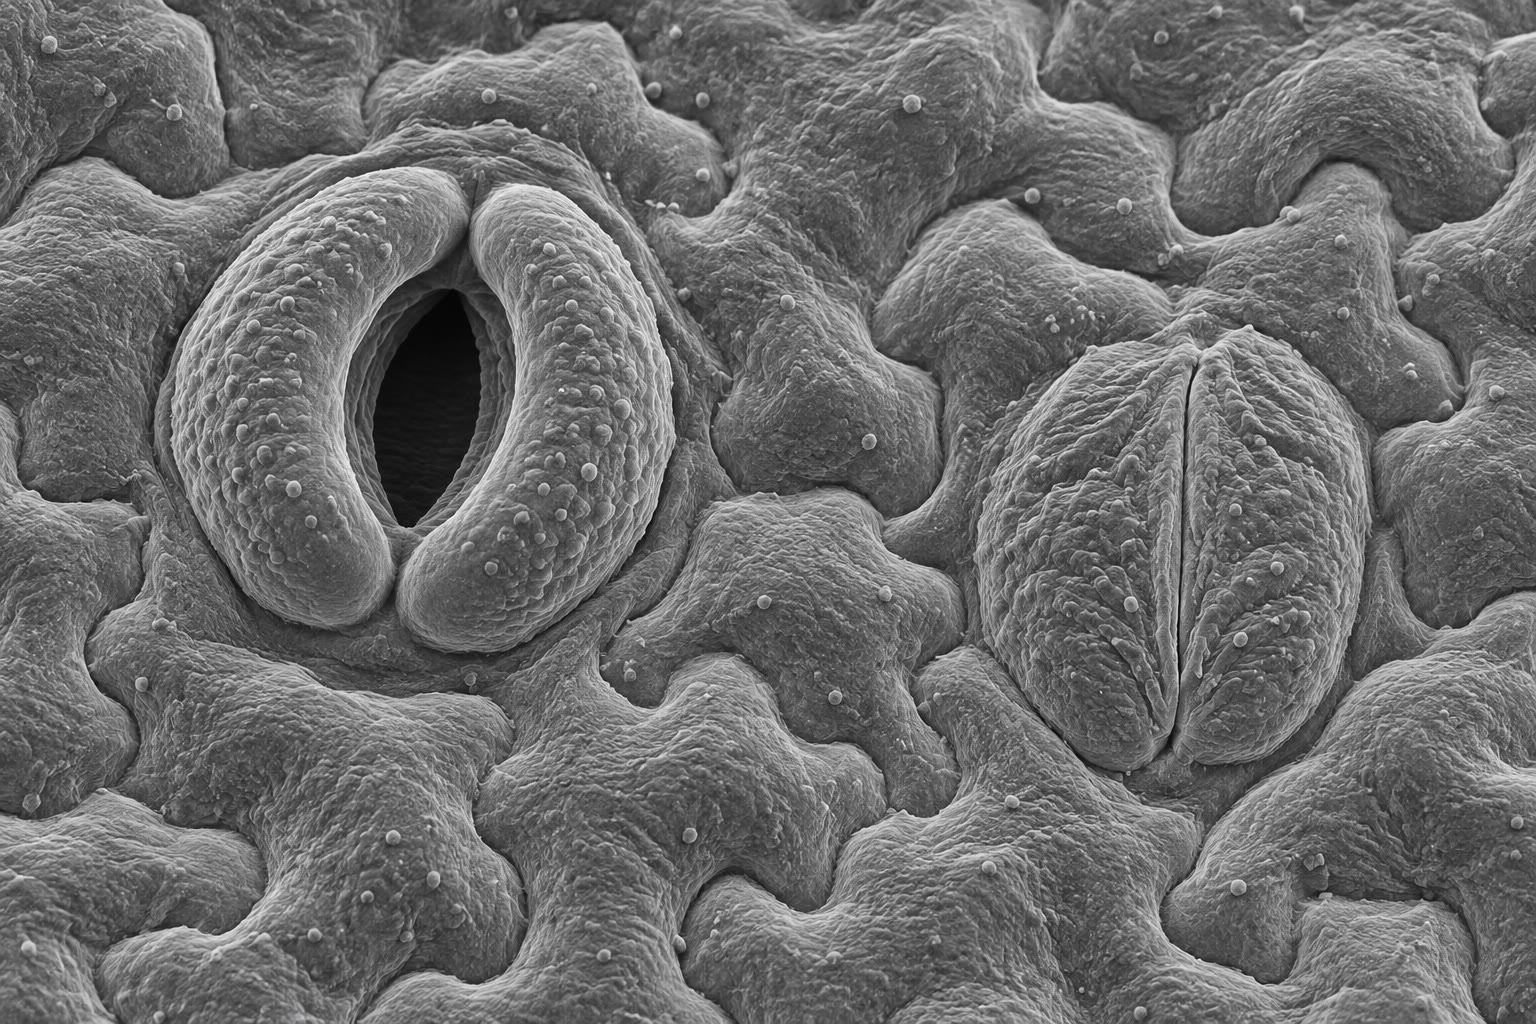
\includegraphics[width=0.46\linewidth]{images/book5/ai/b5-22-stomata-sem.jpg}\hspace{0.04\linewidth}
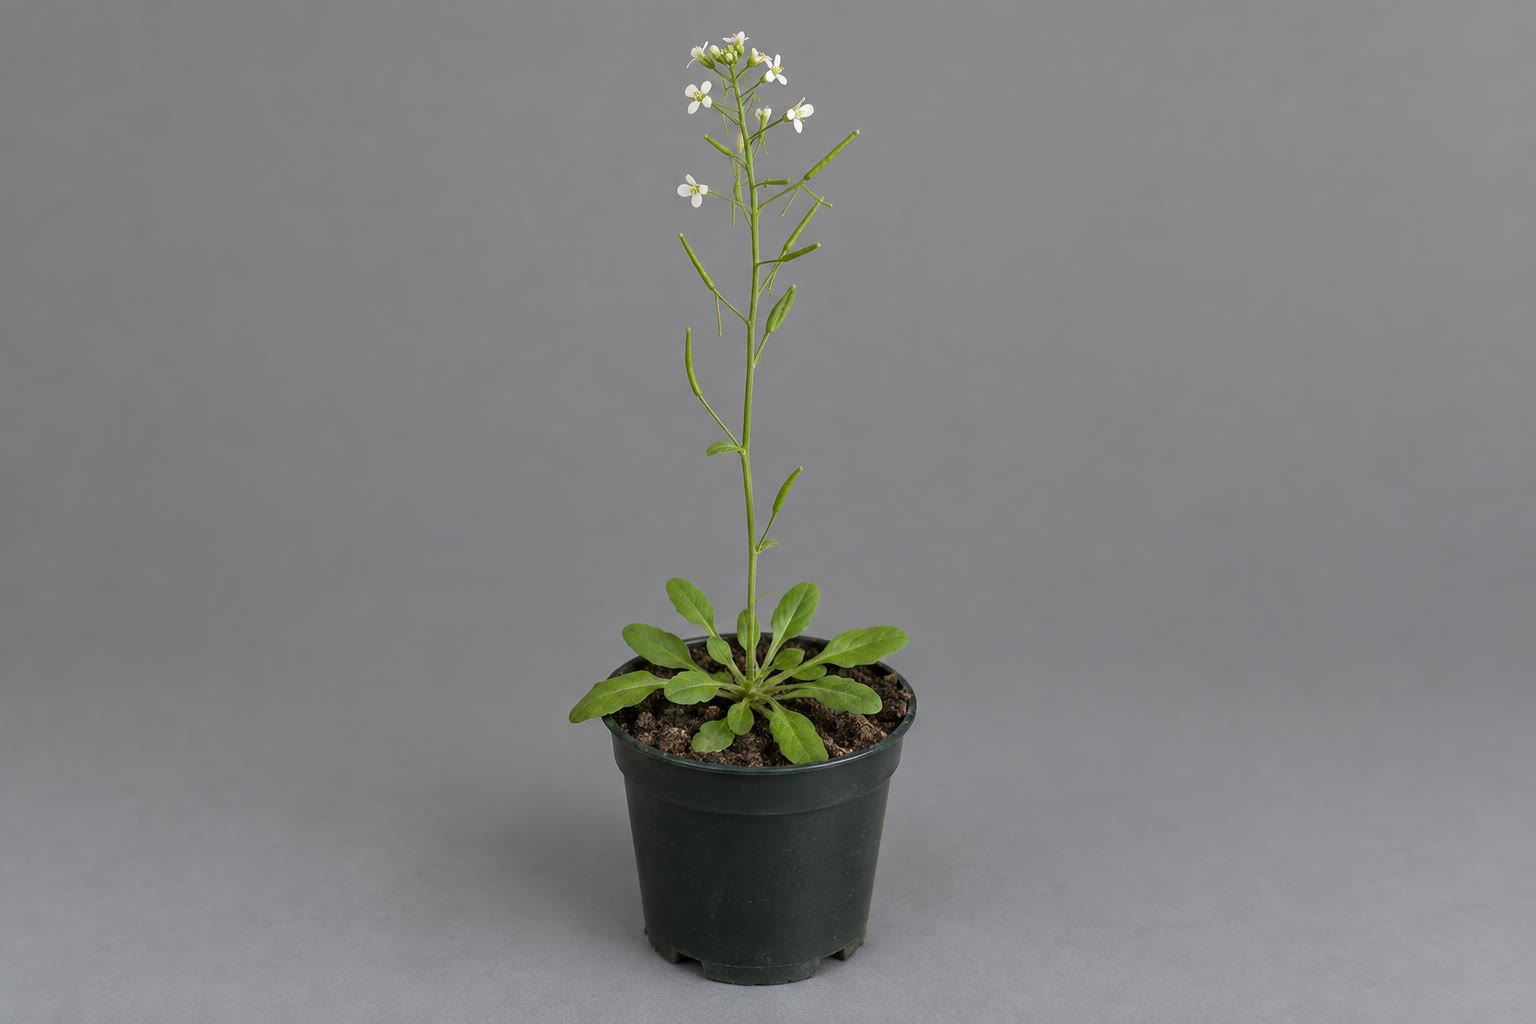
\includegraphics[width=0.46\linewidth]{images/book5/ai/b5-22-arabidopsis.jpg}

{\small 左：叶表面的\omterm{prop:b3:plant-molecular-physiology:stomata}{气孔}，每个孔隙位于其两个
\omterm{prop:b3:plant-molecular-physiology:stomata}{保卫细胞}之间，有的开放，有的关闭。右：\emph{Arabidopsis
thaliana}，一种路边杂草，基因组小，世代周期为六周，
并有十万个突变株系，本章的大多数分子
正是在其中发现的。}
\end{omfigure}

\section{无免疫细胞的免疫}

\begin{definition}[植物免疫的两个层次]\label{def:b3:plant-molecular-physiology:immunity}
\index{模式触发免疫}\index{效应蛋白触发免疫}\index{NLR 受体}\index{超敏反应}\index{系统获得性抗性}\index{水杨酸}\index{茉莉酸}
每个植物细胞本身都是免疫细胞。第一层，
\emph{模式触发免疫}（PTI）依靠表面受体激酶，
识别整类微生物共有的分子——
FLS2 结合细菌鞭毛蛋白的一段 22 个氨基酸，其他受体结合
真菌细胞壁的几丁质片段——并在数分钟内启动
钙离子内流、活性氧爆发、激酶级联、\omterm{prop:b3:plant-molecular-physiology:stomata}{气孔}
关闭、胼胝质沉积使细胞壁加厚，并转录数百个
防御基因；它能阻挡大多数微生物。成功的病原体
会注入\emph{效应蛋白}——能使 PTI 组分失效的蛋白——，
针对这些蛋白的第二层是\emph{效应蛋白触发免疫}
（ETI），由胞内\emph{NLR 受体}（核苷酸结合、
富含亮氨酸的重复序列）承担，每种受体识别一种效应蛋白或其造成的\omterm{def:b3:dna-repair:lesions}{损伤}，
其基因对基因的配对关系由弗洛尔在亚麻锈菌中发现——
（1940 年代）。ETI 比 PTI 更快、更强，通常以
\emph{超敏反应}告终：被感染的细胞及其邻近细胞
自行死亡，将病原体包围在死亡组织中——即抗病叶片上的
小棕斑。两个层次都会释放携带警报信号的\omterm{def:b3:endocrinology:hormone}{激素}：
\emph{水杨酸}针对活体营养型病原体（以活细胞为食），
在整株植物中引发持续数周的\emph{系统获得性抗性}；
\emph{茉莉酸}及\omterm{def:b3:plant-molecular-physiology:hormones}{乙烯}针对\omterm{def:b3:cell-cycle-apoptosis:apoptosis}{坏死}营养型病原体
（先杀死再取食）及咀嚼式昆虫，挥发性
茉莉酸类物质警示邻近植物，并吸引昆虫的
寄生蜂。两种\omterm{def:b3:endocrinology:hormone}{激素}相互拮抗，某些病原体会利用这一点，
例如一种能合成茉莉酸类似物的细菌，会关闭原本能阻止它的
水杨酸防御。
\end{definition}

\begin{omfigure}
\begin{tikzpicture}
\begin{axis}[
  width=0.78\linewidth, height=5.4cm,
  axis x line=bottom, axis y line=left,
  xmin=0, xmax=10, ymin=0, ymax=10,
  xlabel={军备竞赛，从左到右}, ylabel={防御强度},
  xlabel style={font=\small, at={(axis description cs:0.5,-0.08)}, anchor=north}, ylabel style={font=\small},
  xtick=\empty, ytick=\empty,
  clip=false,
]
\addplot[very thick, omDef] coordinates {(0,1) (1.5,5)};
\addplot[very thick, omThm] coordinates {(1.5,5) (3.2,1.8)};
\addplot[very thick, omDef] coordinates {(3.2,1.8) (4.8,8)};
\addplot[very thick, omThm] coordinates {(4.8,8) (6.4,2.2)};
\addplot[very thick, omDef] coordinates {(6.4,2.2) (8.0,8.6)};
\draw[dashed, gray] (axis cs:0,4) -- (axis cs:8.5,4); \node[font=\scriptsize, gray, anchor=west] at (axis cs:8.5,4) {抗性阈值};
\draw[dashed, gray] (axis cs:0,7.2) -- (axis cs:8.5,7.2); \node[font=\scriptsize, gray, anchor=west] at (axis cs:8.5,7.2) {超敏反应};
\node[font=\scriptsize, omDef, anchor=south west] at (axis cs:0.1,5.3) {PTI：受体识别鞭毛蛋白、几丁质};
\node[font=\scriptsize, omThm, anchor=north, align=center] at (axis cs:3.2,1.6) {效应蛋白注入：\\PTI 失效};
\node[font=\scriptsize, omDef, anchor=south, align=center] at (axis cs:4.8,8.2) {ETI：NLR 识别 \\一种效应蛋白};
\node[font=\scriptsize, omThm, anchor=north, align=center] at (axis cs:6.4,2.0) {效应蛋白丢失或改变：\\识别逃逸};
\node[font=\scriptsize, omDef, anchor=south, align=center] at (axis cs:8.0,8.8) {新的 NLR\\演化出现};
\end{axis}
\end{tikzpicture}

{\small 植物与病原体\omterm{prop:b3:bioinformatics:structure}{协同演化}的锯齿状过程。表面受体
针对常见微生物分子引发防御；病原体注入效应蛋白以抑制防御；
植物演化出针对效应蛋白的胞内受体；
病原体丢弃或改变效应蛋白；如此往复，
每一步都会留下抗性与毒力基因，育种者与病原体
至今仍在“交换”这些基因。}
\end{omfigure}

\begin{proof}[证据]
弗洛尔（1940 年代）将亚麻品种与锈菌菌株杂交，发现
对每个菌株的抗性都分离为单个显性植物基因，
其在真菌中对应单个无毒基因——即基因对基因的
关系，在五十年间无法解释，直到首个 NLR 基因于 1994 年被克隆，
并证明首批效应蛋白–受体对能够相互结合，
或标记对方造成的\omterm{def:b3:dna-repair:lesions}{损伤}。戈梅斯-戈梅斯与博勒（2000）发现了
对鞭毛蛋白不起反应的 \emph{Arabidopsis} 突变体 \emph{fls2}，并证明
其受体激酶能以纳摩尔浓度结合肽段 flg22，
该突变体对喷洒在叶面上的细菌更为敏感，
但对注入叶内的细菌则不然——受体守护的是
表面以及细菌进入的\omterm{prop:b3:plant-molecular-physiology:stomata}{气孔}。罗斯（1961）
在一株烟草的一片叶子上接种\omterm{def:b3:virology:virus}{病毒}，发现
一周后其他叶片产生抗性：即\omterm{def:b3:plant-molecular-physiology:immunity}{系统获得性抗性}，后来证明
需要\omterm{def:b3:plant-molecular-physiology:immunity}{水杨酸}参与，而植物合成\omterm{def:b3:plant-molecular-physiology:immunity}{水杨酸}的途径与
阿司匹林母体化合物的途径相同。
\end{proof}

\begin{example}[植物的生物钟与日长]\label{ex:b3:plant-molecular-physiology:clock}
植物拥有与动物生物钟设计相同、但组成部分不相关的\omterm{def:b3:endocrinology:clock}{昼夜节律钟}：
清晨因子（CCA1、LHY）抑制一个傍晚基因（TOC1），
而后者的产物又反过来抑制它们，另有若干反馈环路，使其
即使在持续光照下也能维持稳健的 24 小时循环，并借此预判黎明：
在日出前一小时开放\omterm{prop:b3:plant-molecular-physiology:stomata}{气孔}、开启光合作用基因。
节律钟最重要的输出，是对日长的测量。
在长日植物 \emph{Arabidopsis} 中，生物钟使
CONSTANS 蛋白在午后晚些时候积累；长日条件下，那段午后时光
仍有光照，\omterm{def:b3:plant-molecular-physiology:photoreceptors}{光敏色素}与\omterm{def:b3:plant-molecular-physiology:photoreceptors}{隐花色素}使该蛋白稳定，
它便在叶片中开启 \emph{FT} 基因；短日条件下，
该蛋白在黑暗中合成并被降解。FT 蛋白即成花素，
嫁接实验自柴拉基扬（1936）以来一直在追寻它，它经
韧皮部运至茎尖，并与茎尖中的一个伙伴蛋白共同作用，使茎尖
从产叶转向开花。短日植物（水稻、
大豆）使用同样的生物钟，但信号方向相反。植物由此
通过比较内部节律与外部光照来读取日历——
这便是比宁于 1936 年提出的“外部符合”，并且
七十年后分子遗传学使之成为现实。
\end{example}

\begin{remark}[静止不动，一切皆变]\label{rem:b3:plant-molecular-physiology:remark}
动物应对恶劣环境的办法是离开；植物的办法是
变成另一株植物。它拥有感知光的颜色与方向、
重力牵引、土壤水势、风的触碰，
以及天敌化学信号的受体；它的\omterm{def:b3:endocrinology:hormone}{激素}通过破坏阻遏蛋白起作用，
使一个信号可在数分钟内切换一套程序；
它的每个细胞既是自身的传感器和免疫系统，
必要时又是自身再生的分生组织。养活不断增长世界的矮秆小麦，
其实是一种无法被降解的 \omterm{def:b3:plant-molecular-physiology:hormones}{DELLA} 蛋白；未来几十年的耐旱作物，
很大程度上将取决于 ABA 受体、
\omterm{prop:b3:plant-molecular-physiology:stomata}{气孔导度}，以及
本章所计算的\omterm{prop:b3:plant-molecular-physiology:stomata}{水分利用效率}。
\end{remark}

\section{练习}

\begin{exercise}[$\star$]\label{exo:b3:plant-molecular-physiology:1}
列出三类光感受器及其波长，
并各写出一种响应。植物已有叶绿素，
为何还需要光感受器？
\end{exercise}

\begin{exercise}[$\star$]\label{exo:b3:plant-molecular-physiology:2}
说明\omterm{def:b3:plant-molecular-physiology:hormones}{生长素}、\omterm{def:b3:plant-molecular-physiology:hormones}{赤霉素}与\omterm{def:b3:plant-molecular-physiology:immunity}{茉莉酸}如何共用同一作用机制，
以及这为何使响应迅速。
\end{exercise}

\begin{exercise}[$\star$]\label{exo:b3:plant-molecular-physiology:3}
描述从 ABA 到达\omterm{prop:b3:plant-molecular-physiology:stomata}{保卫细胞}
直至\omterm{prop:b3:plant-molecular-physiology:stomata}{气孔}关闭的事件序列，并指出
在哪一环节发生突变会使植物无法关闭\omterm{prop:b3:plant-molecular-physiology:stomata}{气孔}。
\end{exercise}

\begin{exercise}[$\star$]\label{exo:b3:plant-molecular-physiology:4}
按所识别的对象、受体所在的位置，
以及响应如何结束，区分\omterm{def:b3:plant-molecular-physiology:immunity}{模式触发免疫}与\omterm{def:b3:plant-molecular-physiology:immunity}{效应蛋白触发免疫}。
\end{exercise}

\begin{exercise}[$\star\star$]\label{exo:b3:plant-molecular-physiology:5}
利用拟合式 $\varphi \approx 0.87\,\zeta/(\zeta + 0.6)$，计算
日光下（$\zeta = 1.15$）、单片叶下（$\zeta =
0.4$）、密集冠层下（$\zeta = 0.1$）以及白炽灯下（$\zeta = 0.7$）的
Pfr 比例。为何在此类灯下生长的幼苗会长得高？
\end{exercise}

\begin{exercise}[$\star\star$]\label{exo:b3:plant-molecular-physiology:6}
若细胞壁 pH 为 $5.0$、胞质溶胶 pH 为 $7.5$，计算\omterm{def:b3:plant-molecular-physiology:hormones}{生长素}的胞内外比；
再计算细胞壁酸化至 $4.5$（生长细胞即如此）时的比值。
若在缺氧条件下胞质溶胶酸化至 $6.5$，
其捕获作用会发生怎样的变化？
\end{exercise}

\begin{exercise}[$\star\star$]\label{exo:b3:plant-molecular-physiology:7}
\omterm{def:b3:plant-molecular-physiology:hormones}{生长素}以 \qty{1}{cm/h} 的速度穿过长 \qty{50}{\micro m}
的细胞。它每小时穿过多少个细胞，在每个细胞中停留多长时间？
与扩散 \qty{50}{\micro m} 所需的时间相比较（$D =
\qty{5e-10}{m^2/s}$，$t \approx x^{2}/2D$），并说明
哪一步限制了运输速率。
\end{exercise}

\begin{exercise}[$\star\star$]\label{exo:b3:plant-molecular-physiology:8}
某叶在 \qty{25}{\celsius} 下，内部水蒸气摩尔分数为
\qty{32}{mmol/mol}，空气中为 \qty{16}{mmol/mol}；外部 CO$_{2}$ 为
\qty{400}{ppm}，内部为 \qty{250}{ppm}。计算
每固定一个 CO$_{2}$ 所损失的水分子数。另对 C$_{4}$ 植物，
内部 CO$_{2}$ 为 \qty{150}{ppm}，以及
空气为 \qty{8}{mmol/mol} 的干燥天气，分别重新计算。
\end{exercise}

\begin{exercise}[$\star\star$]\label{exo:b3:plant-molecular-physiology:9}
解释为何经低温驯化的植物往往也更耐旱，
并指出共同的信号与共同的保护性分子。
\end{exercise}

\begin{exercise}[$\star\star\star$]\label{exo:b3:plant-molecular-physiology:10}
\omterm{def:b3:plant-molecular-physiology:photoreceptors}{光敏色素}以速率 $k_{1} + k_{2}$ 趋向其\omterm{prop:b3:plant-molecular-physiology:photoequilibrium}{光平衡}态，
该速率与通量成正比。若全日照下 $k_{1} + k_{2} =
\qty{0.5}{s^{-1}}$，则在黎明时全日照强度的 \qty{1}{\%} 下，
开关切换需要多长时间？Pfr 在黑暗中以半衰期 \qty{2}{h} 回复，
经过 8 小时的夜晚后剩余多少比例，
以及这如何使种子能够区分短暂曝光与整日光照？
\end{exercise}

\begin{exercise}[$\star\star\star$]\label{exo:b3:plant-molecular-physiology:11}
\omterm{def:b3:plant-molecular-physiology:immunity}{超敏反应}每个侵染位点大约杀死一百个细胞。试对一片含
$10^{7}$ 个细胞、每天遭受十次侵染的叶片做粗略的成本–收益估算，
论证为何感染细胞的自杀代价低廉，
以及为何\omterm{def:b3:cell-cycle-apoptosis:apoptosis}{坏死}营养型病原体（以死细胞为食）
会使这一防御成为弱点。
\end{exercise}

\begin{exercise}[$\star\star\star$]\label{exo:b3:plant-molecular-physiology:12}
建立外部符合模型：CONSTANS 蛋白在黎明后第 12 至 16 小时之间合成，
其在黑暗中的半衰期为 \qty{30}{min}，在光照下则为 \qty{4}{h}。
估算在 16 小时日照与 10 小时日照（第 10 小时起为黑暗）下，
第 16 小时时残留的蛋白量，
并说明阈值如何将其转化为开花的决定。
\end{exercise}

\section{问题：阴影下的幼苗}

\begin{problem}[{周末问题——通过分子读取幼苗：冠层下的光敏色素平衡、
所捕获与运输的生长素、经气孔与碳交换的水分，
以及叶片防御的代价，
最终求冠层下的 Pfr 比例、生长素捕获比，
以及水分利用效率}]
\label{pb:b3:plant-molecular-physiology:1}
数据：\omterm{prop:b3:plant-molecular-physiology:photoequilibrium}{光平衡}拟合式 $\varphi = 0.87\,\zeta/(\zeta + 0.6)$；
日光 $\zeta = 1.15$，冠层 $\zeta = 0.2$；下胚轴伸长
速率 $r = r_{0}(1 - \varphi)$，其中 $r_{0} = \qty{2}{mm/h}$。\omterm{def:b3:plant-molecular-physiology:hormones}{生长素}
$\mathrm{p}K_{a} = 4.75$；细胞壁 pH $5.5$，胞质溶胶 pH $7.2$；运输
速度 \qty{1}{cm/h}；细胞长度 \qty{100}{\micro m}。叶片：
内部水蒸气摩尔分数 \qty{32}{mmol/mol}，空气 \qty{16}{mmol/mol}；
外部 CO$_{2}$ \qty{400}{ppm}，内部 \qty{250}{ppm}；$g_{s} =
\qty{0.3}{mol\,m^{-2}\,s^{-1}}$（水蒸气）；叶面积
\qty{20}{cm^2}；\qty{12}{h} 光照。防御：\omterm{def:b3:plant-molecular-physiology:immunity}{超敏反应}
每个位点杀死 $100$ 个细胞；叶片有 $10^{7}$ 个细胞；PTI
活跃时耗费 \qty{5}{\%} 的光合作用。

\medskip
\noindent\textbf{第一部分——光。}
\begin{enumerate}
  \item 计算日光下和冠层下的 $\varphi$。
  \item 两种条件下的伸长速率，以及
        遮荫中经过 \qty{48}{h} 后多出的长度。
  \item 相邻植株的一片叶子去除了日光中 \qty{90}{\%} 的红光，以及
        \qty{20}{\%} 的远红光。计算新的 $\zeta$
        和 $\varphi$。单片叶子是否足以触发
        \omterm{prop:b3:plant-molecular-physiology:photoequilibrium}{避荫}反应？
  \item 解释为什么 $\varphi$ 与亮度无关，以及
        这对于开阔处阴天里的幼苗意味着什么。
  \item 全日照下 $k_{1} + k_{2} = \qty{0.5}{s^{-1}}$。达到\omterm{prop:b3:plant-molecular-physiology:photoequilibrium}{光平衡}的
        \qty{95}{\%} 所需时间，以及达到
        \qty{1}{\%} 所需时间各为多少？
  \item 白天生成的 Pfr 以半衰期 \qty{2}{h} 回复。
        经过 \qty{8}{h} 和 \qty{14}{h} 黑暗后剩余的比例各为多少；
        植物如何能将其用作夜长计时器，
        以及它为什么是一个较差的计时器？
\end{enumerate}

\medskip
\noindent\textbf{第二部分——\omterm{def:b3:plant-molecular-physiology:hormones}{生长素}。}
\begin{enumerate}[resume]
  \item 细胞壁和胞质溶胶中呈中性的 IAAH
        占\omterm{def:b3:plant-molecular-physiology:hormones}{生长素}的比例。
  \item 平衡时 IAAH 的内外比。若细胞壁中
        \omterm{def:b3:plant-molecular-physiology:hormones}{生长素}总量为 \qty{0.1}{\micro M}，
        求胞质溶胶中的浓度。
  \item 每小时穿过的细胞数，以及每个细胞中的停留时间。
  \item 一段长 \qty{5}{cm} 的茎：茎尖\omterm{def:b3:plant-molecular-physiology:hormones}{生长素}的变化
        要多久才能传到基部？与茎开始向光弯曲所需的一小时相比较，
        并加以评论。
  \item 在重力刺激的根中，PIN3 重新定位，使下侧
        接收 \qty{60}{\%} 的流量，上侧
        接收 \qty{40}{\%}。若根细胞伸长在\omterm{def:b3:plant-molecular-physiology:hormones}{生长素}
        高于常规水平时每高出 \qty{1}{\%} 即下降 \qty{1}{\%}，低于常规水平时同样幅度上升，
        计算两侧相对于常规的速率，
        以及弯曲的方向。
  \item 为什么同样的不对称使茎向相反方向弯曲？
\end{enumerate}

\medskip
\noindent\textbf{第三部分——以水换碳。}
\begin{enumerate}[resume]
  \item 以 \unit{mmol\,m^{-2}\,s^{-1}} 为单位的蒸腾 $E = g_{s}\,\Delta w$。
  \item 同化 $A = (g_{s}/1.6)\,\Delta c$，单位为 \unit{\micro
        mol\,m^{-2}\,s^{-1}}，以及比值 $E/A$。
  \item \qty{20}{cm^2} 叶片在 12 小时白天中散失的水量，以
        摩尔和克计；固定的碳，以 CO$_{2}$ 的摩尔数和
        葡萄糖的克数计。
  \item ABA 使\omterm{prop:b3:plant-molecular-physiology:stomata}{气孔}关闭至 $g_{s} = \qty{0.05}{}$。求新的 $E$ 和
        $A$，以及比值。植物得到了什么，又失去了什么？
  \item C$_{4}$ 植物内部 CO$_{2}$ 保持在 \qty{150}{ppm}，
        $g_{s}$ 不变时，其 $E/A$ 是多少？CAM 植物在夜间
        开放，此时 $\Delta w = \qty{5}{mmol/mol}$，其 $E/A$ 在 $\Delta c =
        \qty{150}{ppm}$ 时是多少？
  \item 解释比值 $E/A$ 为什么与 $g_{s}$ 无关，以及
        植物对此能做什么、不能做什么。
\end{enumerate}

\medskip
\noindent\textbf{第四部分——防御。}
\begin{enumerate}[resume]
  \item 每天十个感染位点，每个都以\omterm{def:b3:plant-molecular-physiology:immunity}{超敏反应}应对；
        被杀死的细胞数（每天），以占叶片的比例表示。
  \item 叶片寿命为 60 天，牺牲的比例是多少？与之比较，
        若十次感染中有一次逃脱并每次摧毁叶片的
        \qty{5}{\%}，其损失如何？
  \item PTI 活跃的时间占 \qty{20}{\%}：平均代价
        占光合作用的比例。为什么植物不让它始终保持开启？
  \item 病原体删除了 NLR 所识别的效应蛋白。它得到了什么，
        失去了什么，以及植物种群接下来
        会怎样？
  \item 一种细菌分泌\omterm{def:b3:plant-molecular-physiology:immunity}{茉莉酸}模拟物。它关闭了哪一种防御，
        以及这为何对它有利，鉴于
        两条\omterm{def:b3:endocrinology:hormone}{激素}途径之间的拮抗关系？
  \item 为什么单一作物中的基因对基因抗性常在
        几季之内被攻破，而锯齿形曲线提示育种者
        应改用什么方法？
  \item 总结：冠层下的 $\varphi$（第 1 题）、\omterm{def:b3:plant-molecular-physiology:hormones}{生长素}
        捕获比（第 8 题）以及每固定一个
        CO$_{2}$ 所失去的水分子数（第 14 题）。
\end{enumerate}
\end{problem}
